%!TEX encoding = IsoLatin
%!TEX root = ./rapport.tex
\section{Annexes}

\subsection{Budget}

\begin{table}[htdp]
\begin{center}
\begin{tabular}{|l|l|}
\hline Libell� & Prix\\
\hline \hline Aimants & \EUR{24.80}\\
\hline Plaque de cuivre & \EUR{23.20}\\
\hline Isolant & \EUR{12.05}\\
\hline Corde & \EUR{3.67} \\
\hline Poulie & \EUR{3.05} \\
\hline Porte-v�lo & \EUR{50} \\
\hline \hline Total & \EUR{116,67} \\
\hline
\end{tabular}
\end{center}
\end{table} 

%\subsection{Mesure du champ d'un aimant}
%
%Soit $w_{m}$ la densit� de l'�nergie m�canique.
%
%$$w_{m}=\frac{1}{2\mu_{0}}B^{2}$$
%O� $\mu_{0}=4\pi 10^{-7}$ est la perm�abilit� magn�tique du vide.\\
%$w_{M}$ est l'�nergie m�canique et est donc d�finie par :
%
%$$w_{M}=w_{m}V=\frac{1}{2\mu_{0}}B^{2}V$$
%O� $V$ est le volume de l'entre-fer.\\
%Quand deux aimants sont coll�s l'un � l'autre, $V=0$, donc $w_{M}=0$
%
%\begin{figure}[H] %on ouvre l'environnement figure
%	\centering
%	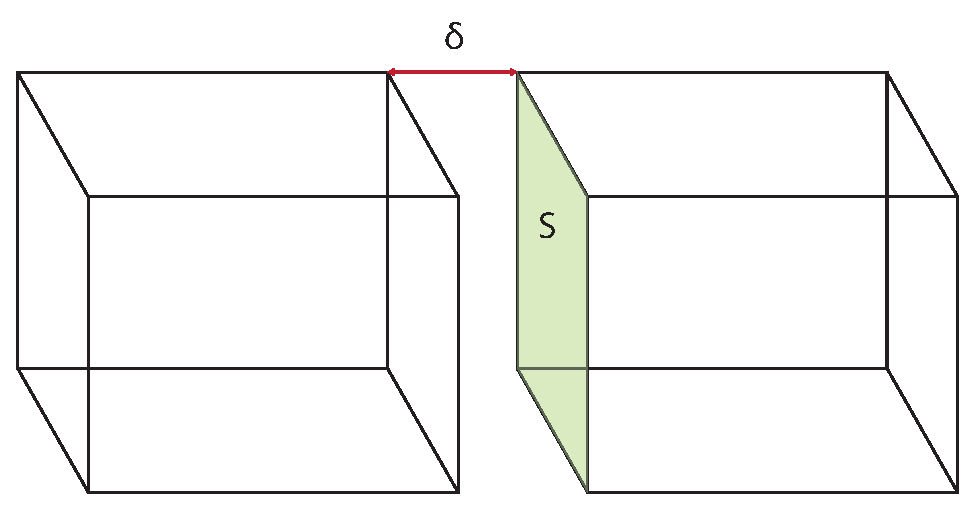
\includegraphics[width=10cm]{schema6.eps} %ou image.png, .jpeg etc.
%	\caption{\small Entre-fer des aimants.} %la l�gende
%	\label{aimants} %l'�tiquette pour faire r�f�rence � cette image
%\end{figure} %on ferme l'environnement figure
%
%Quand ces deux aimants sont espac�s d'une longueur $\delta$, (Figure~\ref{aimants})
%
%$$w_{M}=\frac{1}{2\mu_{0}}B^{2}S\delta$$
%
%O� S est la surface de l'entre-fer. ($V=S\delta$)
%
%Or, l'�nergie m�canique est aussi (travail) : $w_{M}=F_{M}\delta$
%
%Donc : $$F_{M}=\frac{1}{2\mu_{0}}B^{2}S$$
%
%Il suffit ensuite d'isoler $B$ en fonction de la force exerc�e sur un des aimants pour les s�parer :
%
%$$B=\sqrt{\frac{2F_{M}\mu_{0}}{S}}$$

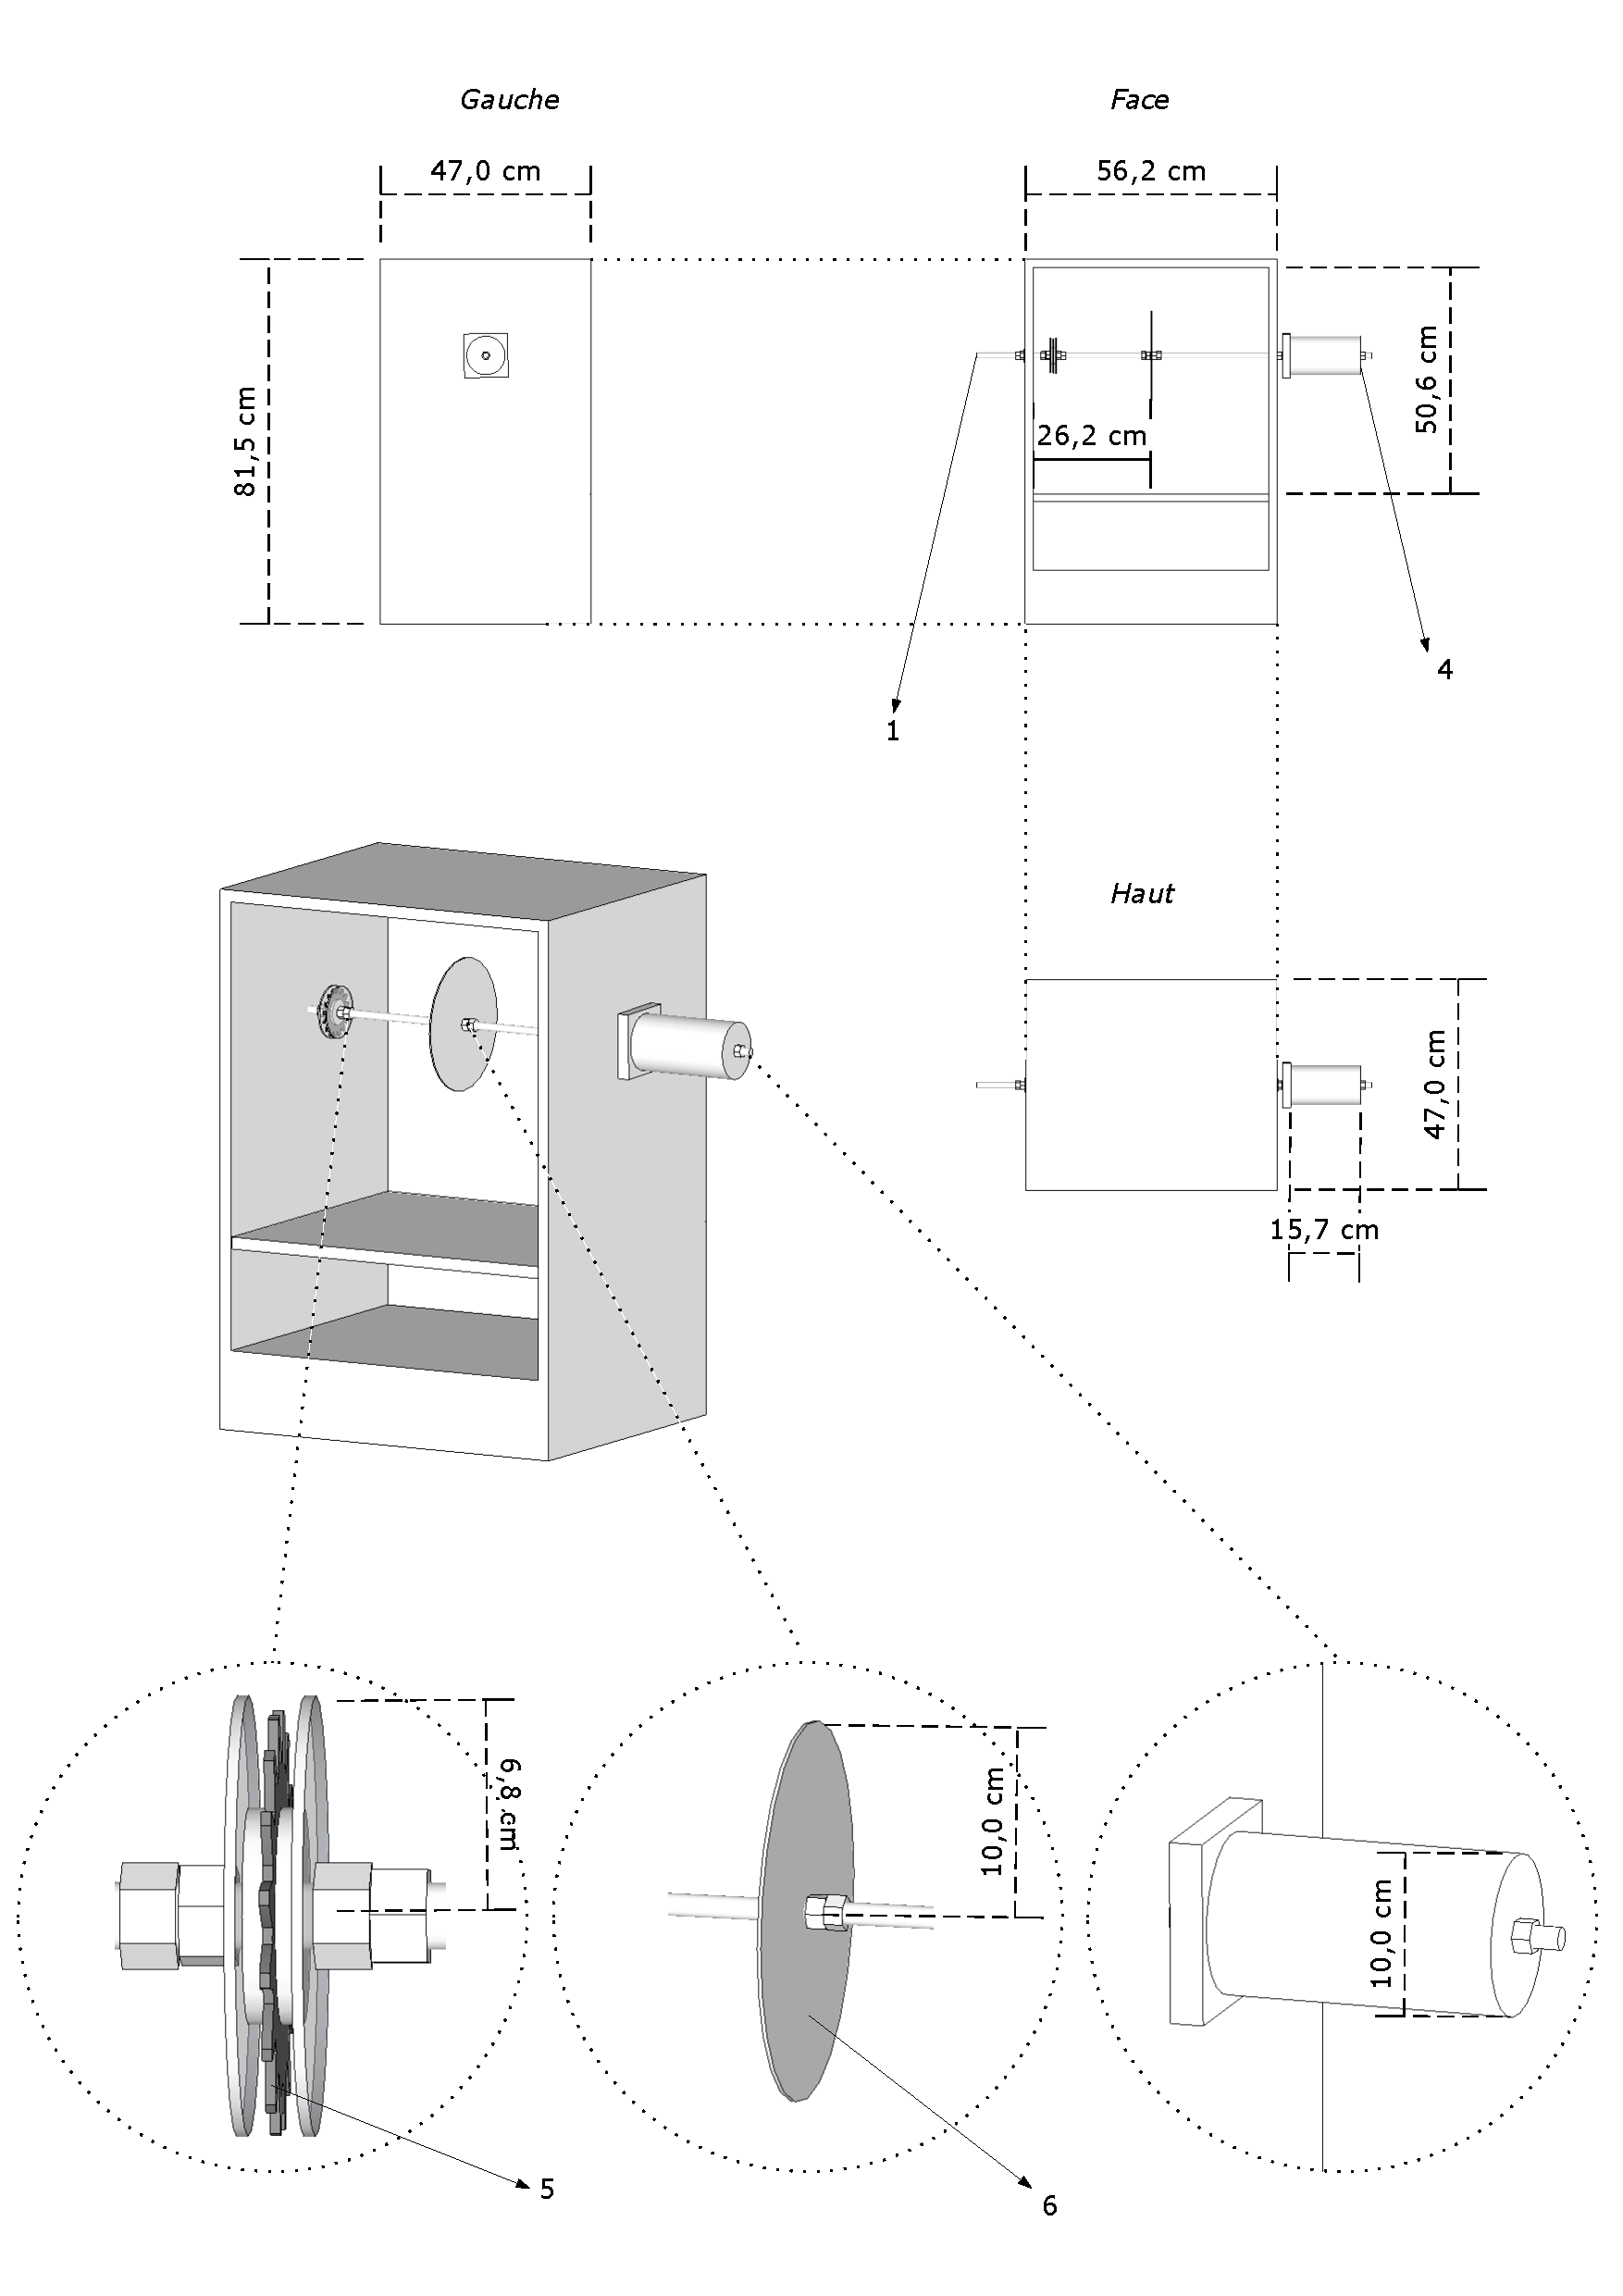
\includepdf{plan1.pdf}
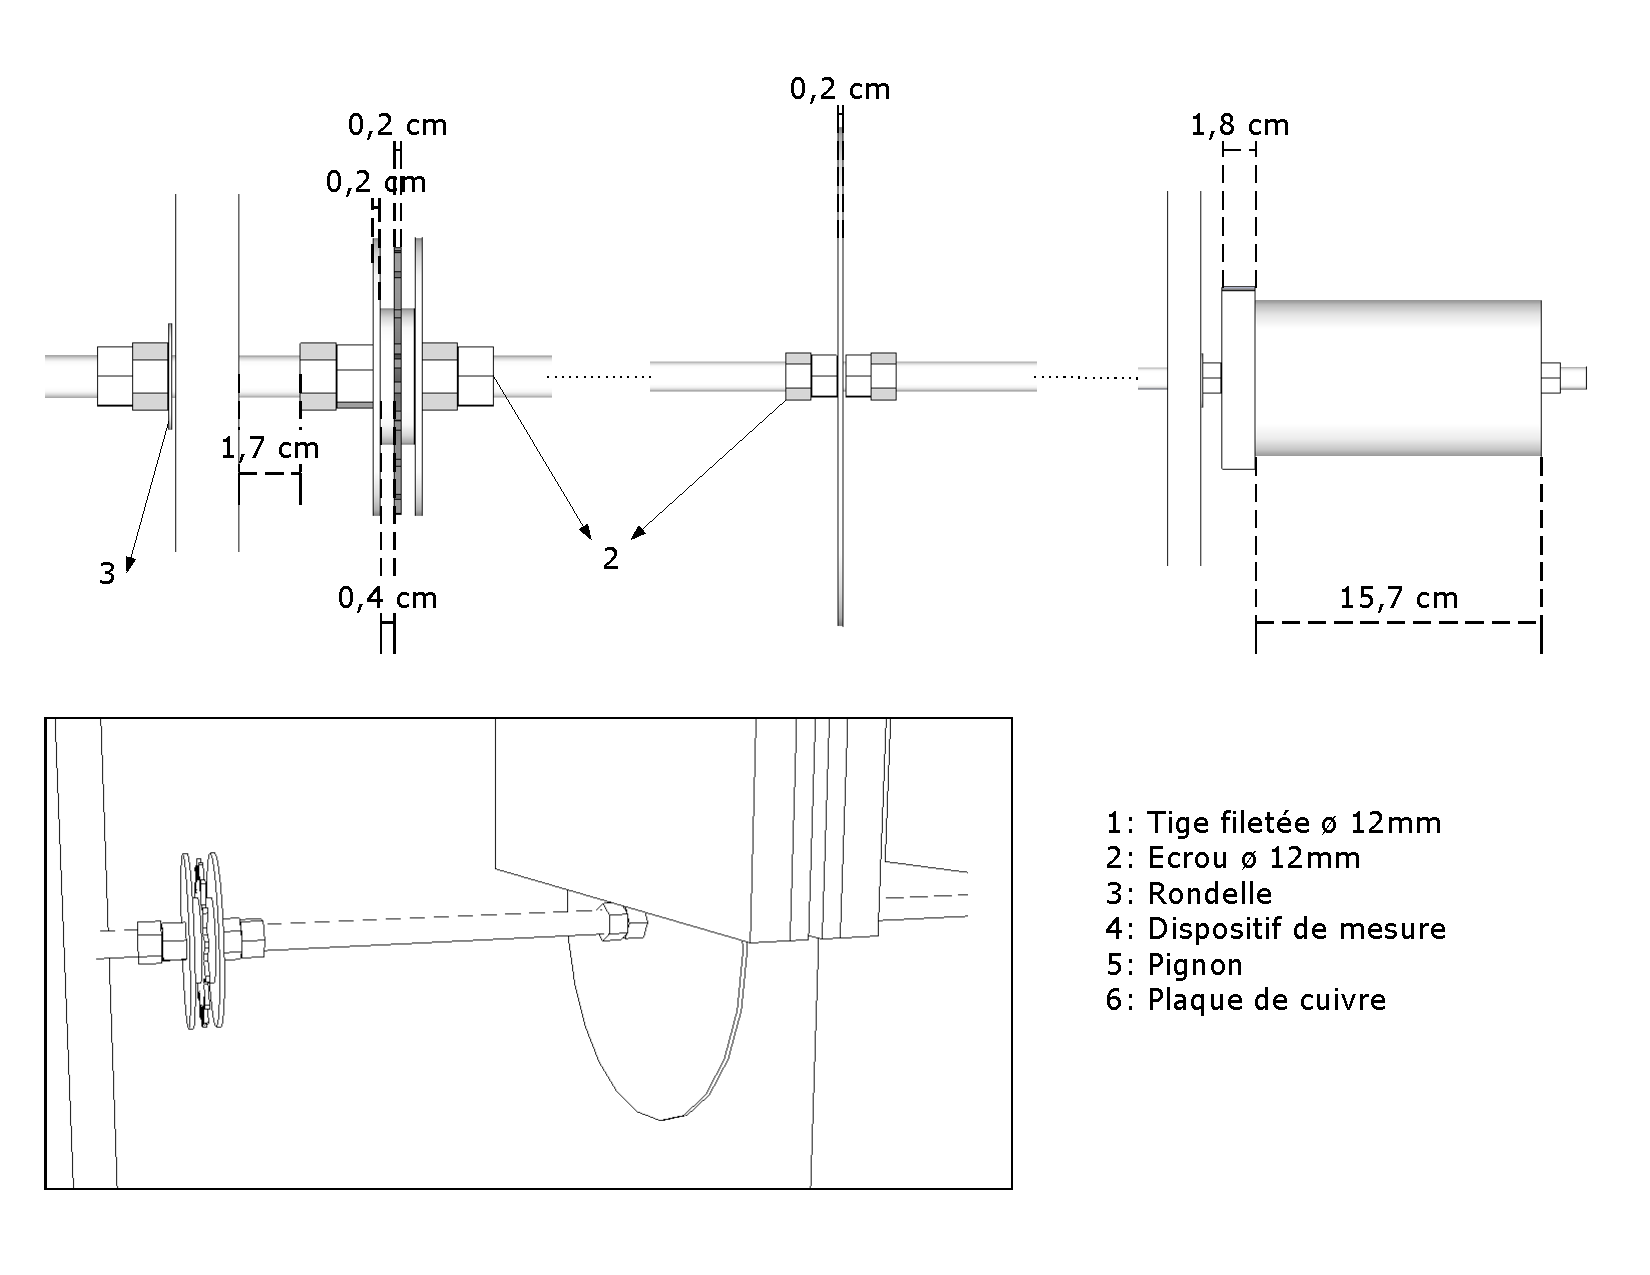
\includepdf[fitpaper]{plan2.pdf}

%\subsection{Photos}

%\begin{figure}[H] %on ouvre l'environnement figure
%	\centering
%	\includegraphics[width=10cm]{roulement.eps} %ou image.png, .jpeg etc.
%	\caption{\small R�cup�ration de roulements � bille pour soutenir l'axe} %la l�gende
%	\label{roule} %l'�tiquette pour faire r�f�rence � cette image
%\end{figure} %on ferme l'environnement figure
